
\chapter{Risultati}

\section{Velocità in lettura}

\begin{figure}[htbp]
    \begin{center}
        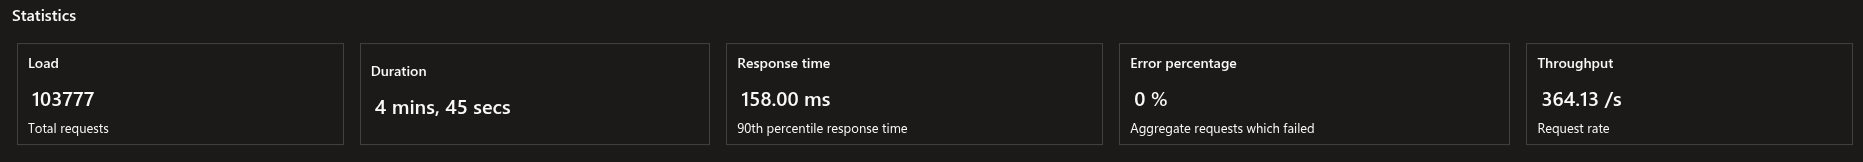
\includegraphics[width=\textwidth]{TestLettura1.png}
        \caption{158 ms su una media di 364 richieste al secondo}
    \end{center}
\end{figure}

\begin{figure}[htbp]
    \begin{center}
        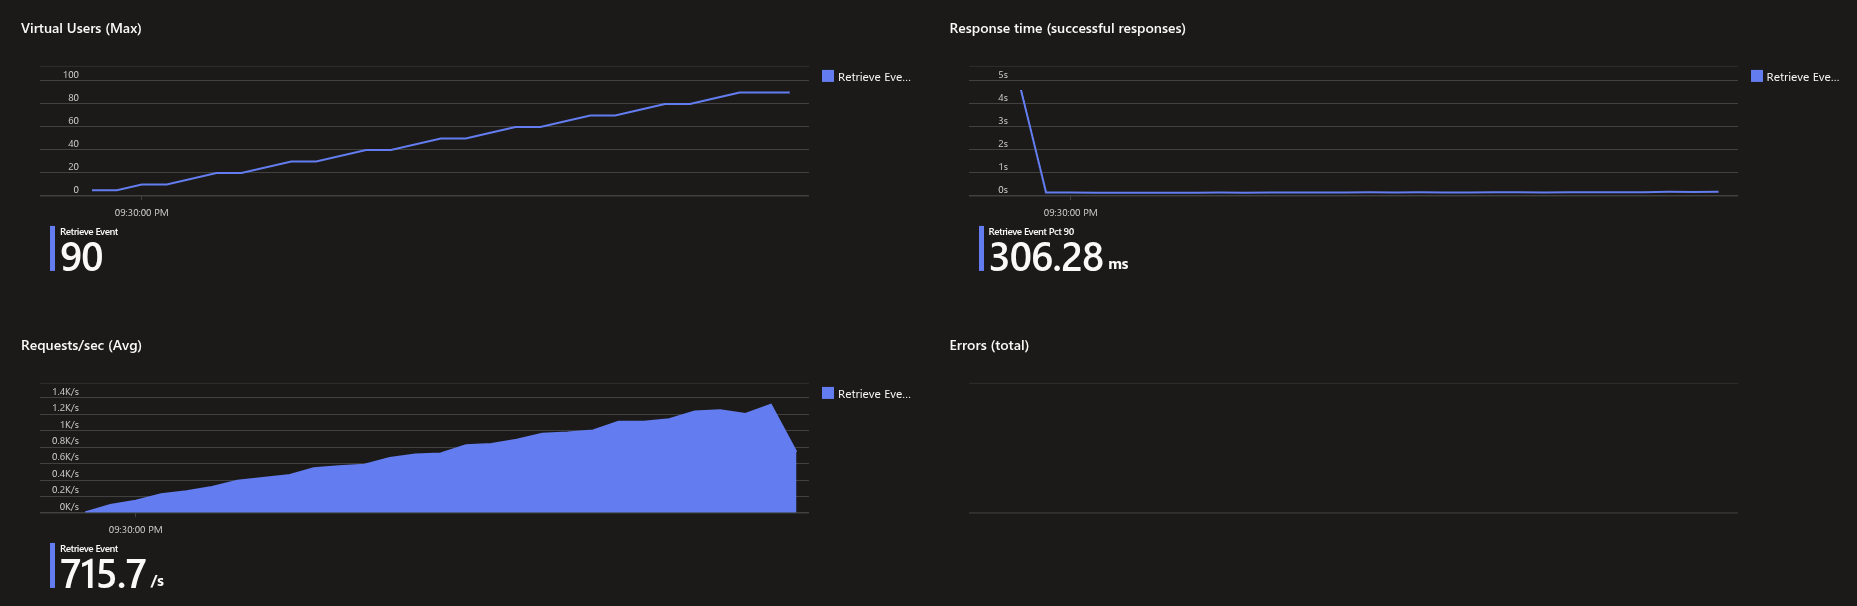
\includegraphics[width=\textwidth]{TestLettura2.png}
        \caption{il tempo di risposta non varia in base al numero di richieste}
    \end{center}
\end{figure}

\begin{figure}[htbp]
    \begin{center}
        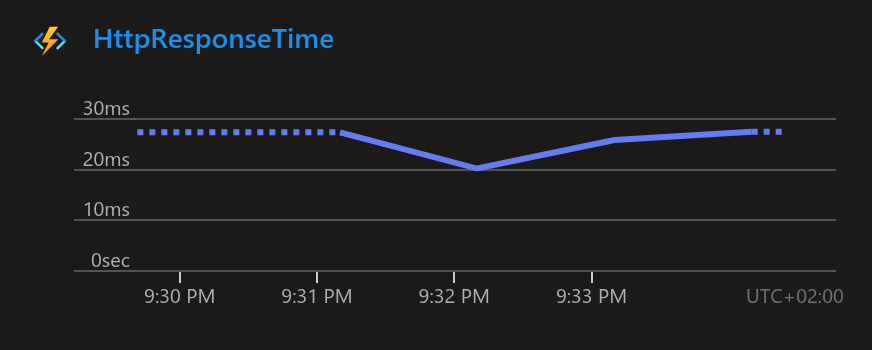
\includegraphics[width=\textwidth]{TestLettura3.png}
        \caption{Dettaglio della velocità senza tempo di trasmissione}
    \end{center}
\end{figure}
\clearpage
\section{Caricamento di immagini concorrenti}

\begin{figure}[htbp]
    \begin{center}
        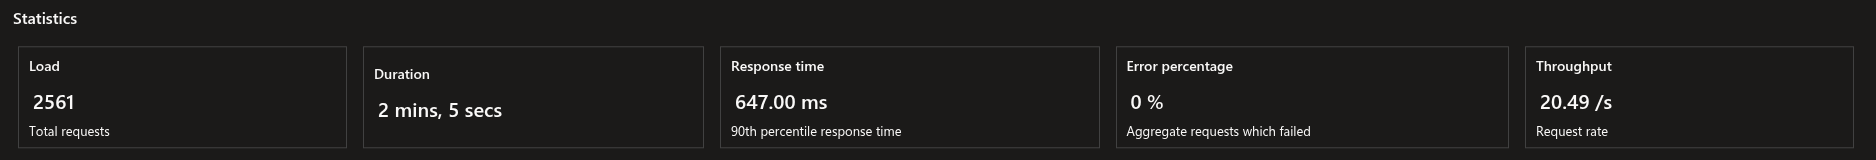
\includegraphics[width=\textwidth]{UploadImages1.png}
        \caption{2 MB di immagini in 600 ms 20 volte al secondo}  
    \end{center}
\end{figure}

\begin{figure}[htbp]
    \begin{center}
        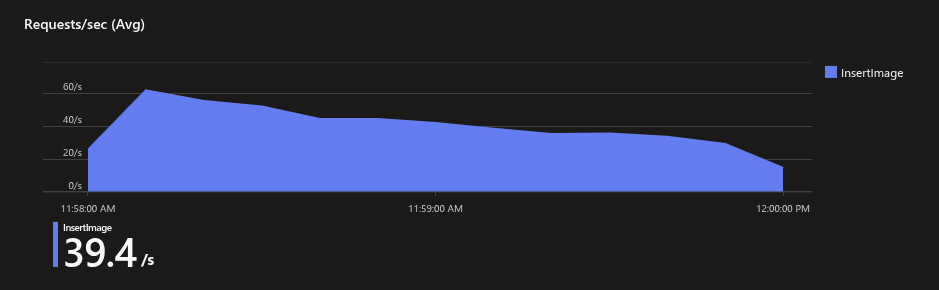
\includegraphics[width=\textwidth]{UploadImages3.png}
        \caption{Andamento delle richieste}  
    \end{center}
\end{figure}

\begin{figure}[htbp]
    \begin{center}
        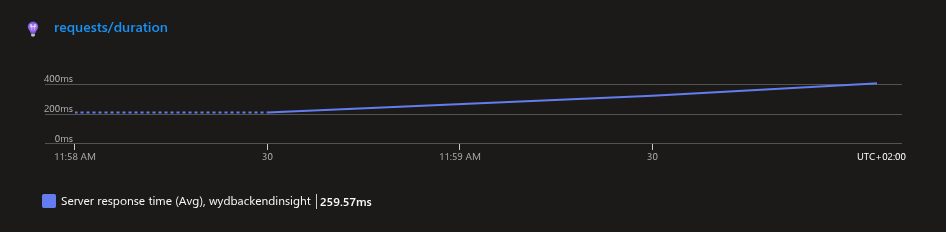
\includegraphics[width=\textwidth]{UploadImages2.png}
        \caption{Dettaglio della velocità richiesta dal server}
    \end{center}
\end{figure}


\clearpage
\chapter*{Conclusione}
\addcontentsline{toc}{chapter}{Conclusione}

\begin{figure}[htbp]
    \begin{center}
        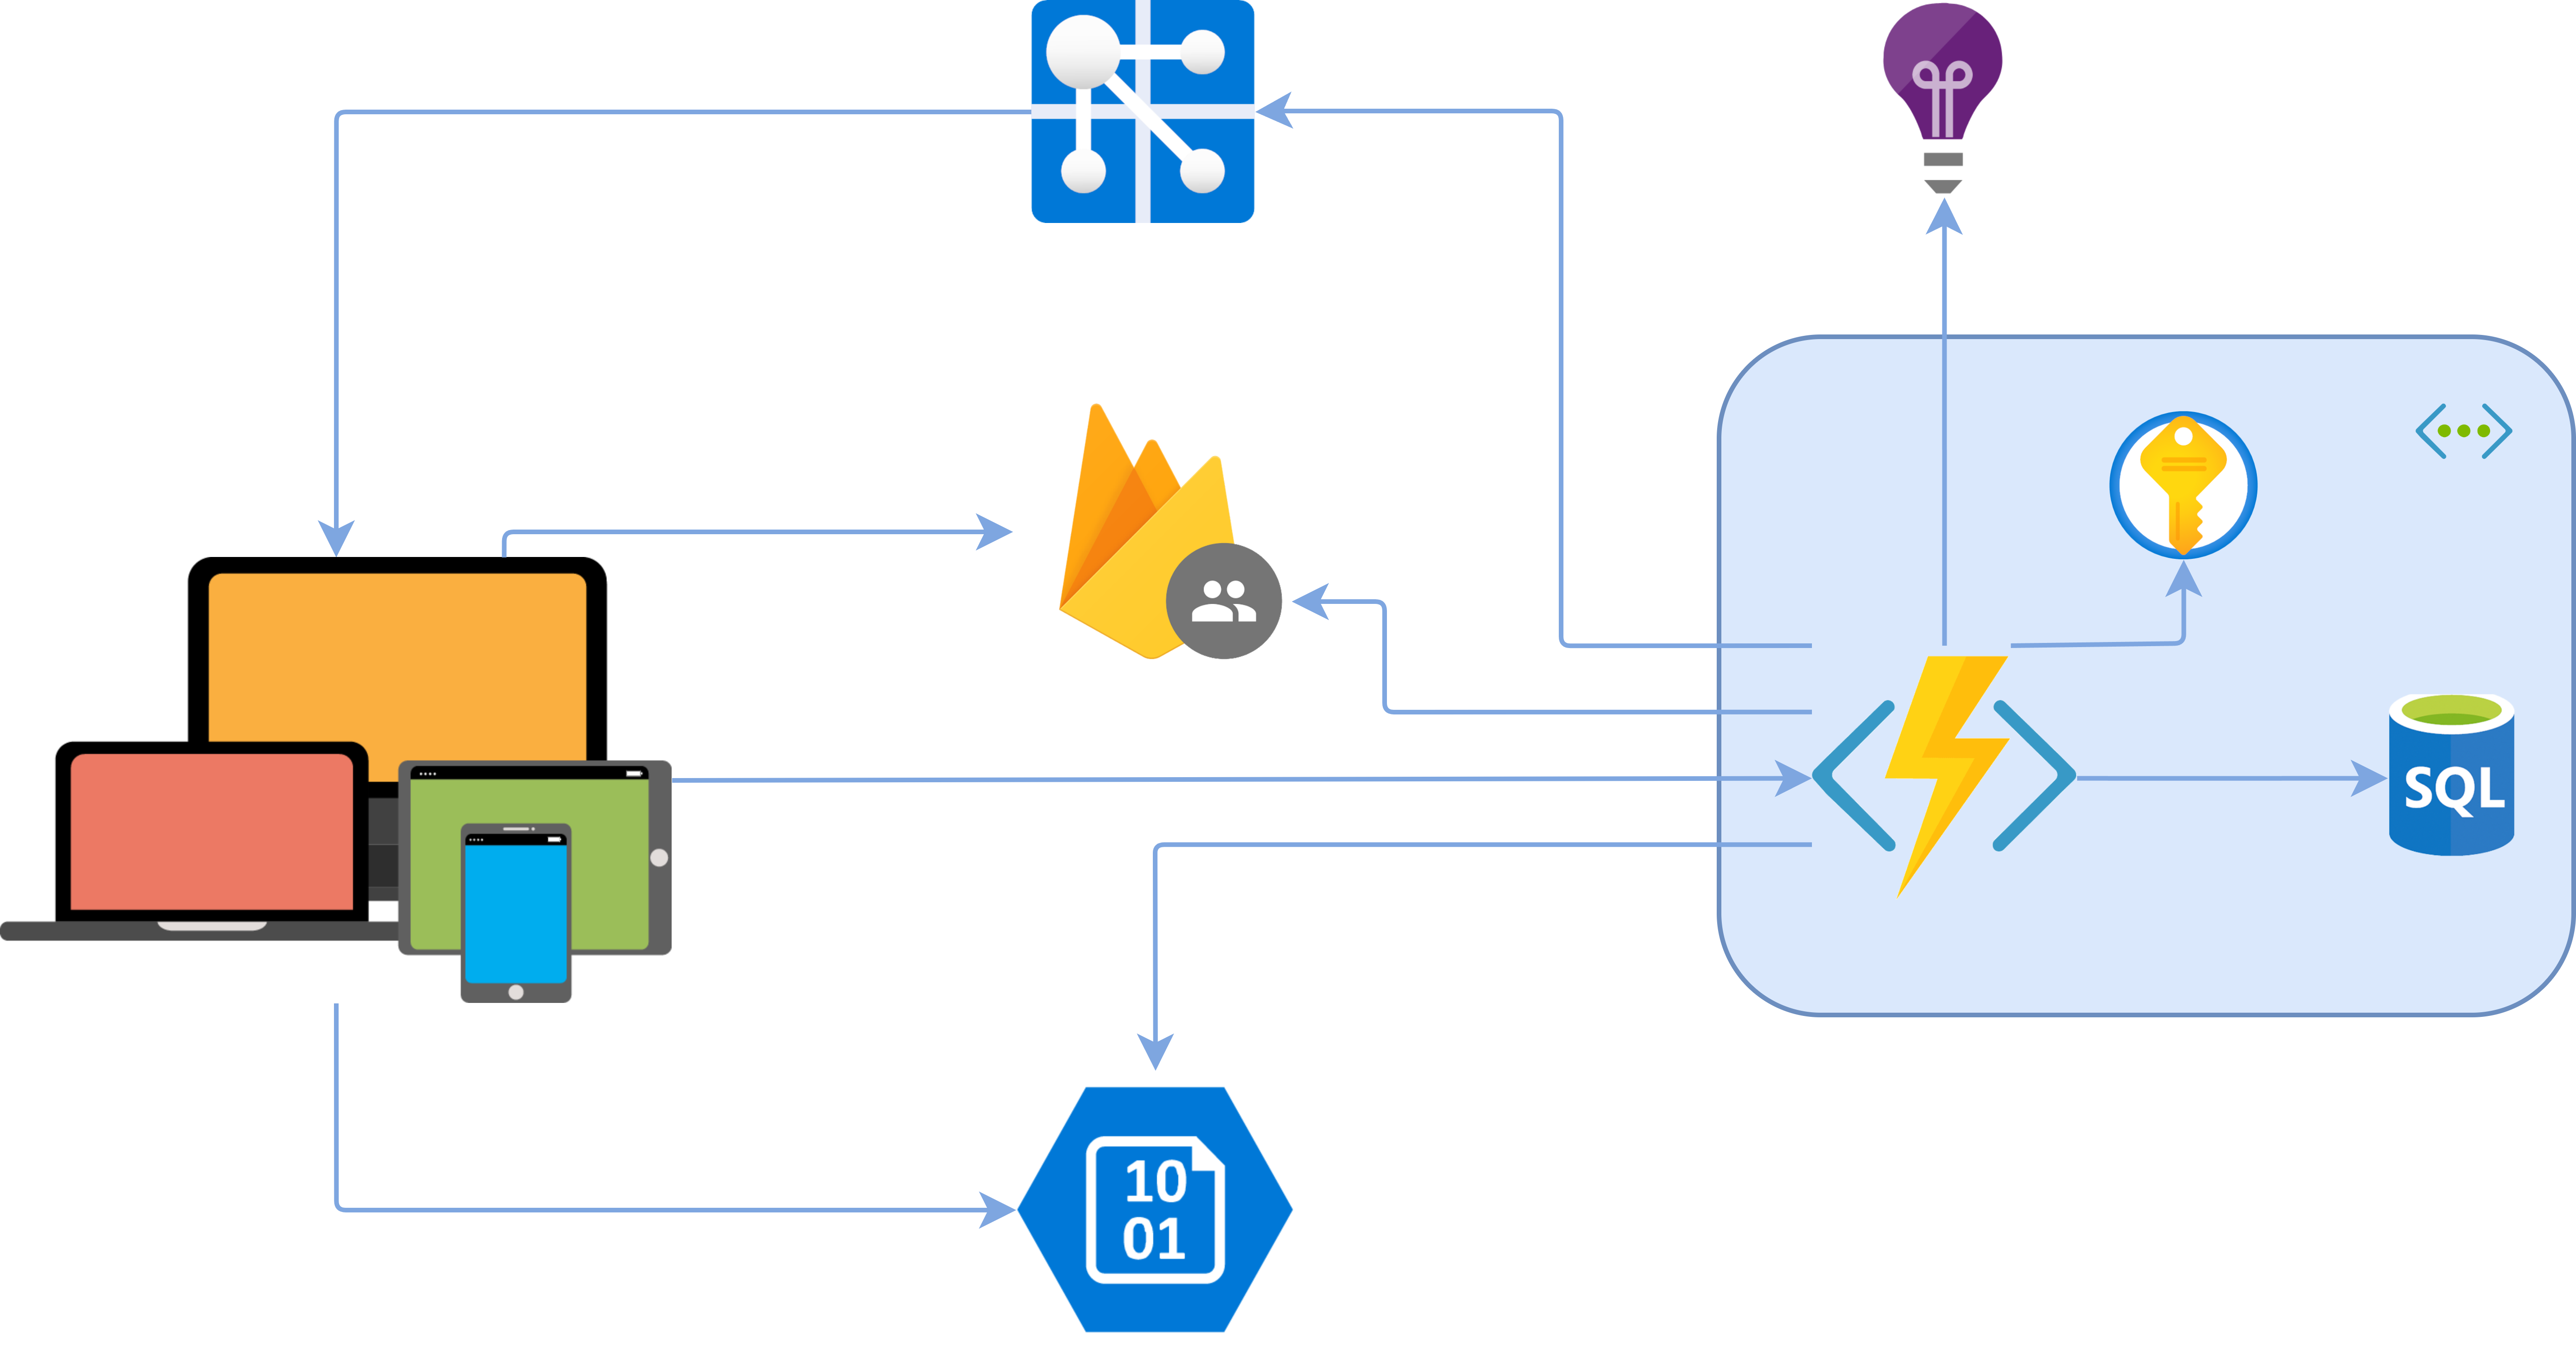
\includegraphics[width=\textwidth]{ImplementazioneArchitettura.png}
        \caption{Grafico dell'architettura finale}
    \end{center}
\end{figure}
\clearpage

\section{Sviluppi futuri}
Gli sviluppi futuri potranno comprendere, in base a decisioni di marketing:
\begin{itemize}
    \item La visualizzazione degli impegni degli altri profili
    \item L'implementazione di una chat per ogni gruppo
    \item Sviluppo di strumenti utili all'organizzazione dei gruppi, quali:
          \begin{itemize}
              \item form per combinare le disponibilità reciproche
              \item appunti condivisi(liste della spesa o note su chi porta cosa)
              \item calcolo delle spese compiute da ciascun componente
          \end{itemize}
    \item La creazione di profili pubblici che possono essere seguiti
    \item La creazione di eventi pubblici
    \item Una funzionalità di ricerca degli eventi o dei profili pubblici
    \item Supporto alla gestione di prenotazione e organizzazione degli eventi, dalle liste di attesa alla vendita dei biglietti
    \item La possibilità per le aziende di gestire in locale il proprio server e i relativi dati
\end{itemize}
\clearpage

\chapter*{Fonti bibliografiche e sitografia}
\addcontentsline{toc}{chapter}{Fonti bibliografiche e sitografia}

Object Management Group, OMG Unified Modelling Language Version 2.5.1, December 2017, https://www.omg.org/spec/UML/2.5.1/PDF
